\section{Log replication and commitment}
\label{related:logreplication}

All consensus algorithms specify how to send new log entries to other
servers and when to mark them committed. This is usually done in one
round of communication from the leader in the normal case, and it is
usually straightforward to apply batching and pipelining to make
replicating multiple entries faster.

The algorithms differ in how far they can proceed out of order. Raft,
Zab, and Viewstamped Replication must all append and commit entries to
the log in order, so that followers' logs always remain consistent with
the leader's. Traditionally, Multi-Paxos allows servers to accept and
commit values for entries in any order. This does not offer Paxos a
significant performance advantage, however, since commands must still be
applied to the state machines in order. Raft and the other algorithms
that maintain a log in order can also transmit log entries out of
order; they just cannot be appended to the log this way. (In these
algorithms, servers could buffer the entries outside the log until they
are ready to be appended, if desired.)

\begin{figure}
\centering
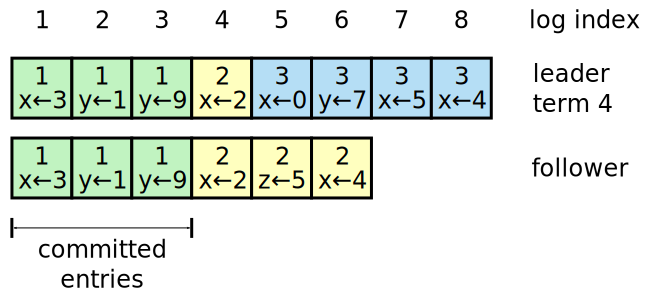
\includegraphics[scale=.50]{related/rereplicate}
\vcaption[differences in how new leaders replicate existing entries]{
Example of how algorithms differ in which entries a new leader
replicates from its log. In Paxos, the new leader for term~4 executes
phases~1 and~2 of Paxos for entries 4--8 using its new proposal number,
since it does
not believe that those are committed. As described in the Viewstamped
Replication and Zab papers, the new leader replicates its entire log to
the follower. In Raft, the leader only transmits entries 5--8 to the
follower, the minimal number of entries required.
}
\label{fig:related:rereplicate}
\end{figure}

The algorithms also differ in what new leaders do with existing entries
in their logs, as illustrated in Figure~\ref{fig:related:rereplicate}:
%
\begin{itemize}
%
\item In Paxos, a new leader goes through the two phases of
single-decree Paxos for each uncommitted entry it finds, rewriting and
renumbering them all with its current proposal number. This either
commits the local value or discovers an existing committed value.
Meanwhile, it can replicate and commit but not yet apply client commands
in further log slots.
%
\item In Viewstamped Replication Revisited and Zab, a new leader
transfers its entire initial log to each follower before starting its
term, and the entire log is effectively renumbered with the new view.
This is impractical for large logs and should be optimized to send fewer
entries in practice, but the details have not been published. It is
fairly easy to determine which entries to send if the two servers both
participated in the last view but more difficult to determine otherwise
(without the term numbers in each entry as in the figure, one idea would
be to compare cumulative hashes of log prefixes).
%
\item
A new leader in Raft transfers just the minimal number of entries to
make other servers' logs match its own. After some back-and-forth with
heartbeats to discover where the logs diverge, the only entries that are
transferred are those that differ.
%
Key to this feature is that entries are not renumbered, so the same
entry will have the same index and term across logs for all time.
Without this property, some servers would have an entry under its
original term number, and others would have it under new term numbers. A
subsequent leader would have to needlessly overwrite some of these
copies, since it wouldn't know which ones contain the same command.
%
\end{itemize}

By transferring log entries rather than logs, Raft allows more
intermediate states than VR and Zab. These intermediate states
are ambiguous in Raft, thus cannot be used for commitment (see
Figure~\ref{fig:basicraft:oldTermCommit}). This has three
consequences.

First, if we could somehow observe a snapshot of an entire cluster, an
entry in Raft can be present on a majority of servers but not committed.
Instead, to determine whether an entry is committed, one must ask if
future leaders must have the entry: does every server that could be
elected leader with its current log have the entry in its log? If so,
the entry is committed; otherwise, it is not. This requires more complex
reasoning for an omniscient observer than in other algorithms: rather
than counting how many replicas of the entry exists, one must
essentially execute the consensus algorithm.

Second, during operation, Raft has a two-part commitment rule, in which
entries from prior terms are not directly marked committed; they are
only marked committed once an entry from the current term has reached a
majority of the cluster (at this point, any ambiguity is resolved). This
does not significantly burden implementations, which only need a single
additional \emph{if} statement. Interestingly, this commitment rule
would not be possible in a single-decree consensus formulation; it
relies on the log formulation so that later entries can commit earlier
ones.

Finally, infinite leader changes can require infinite space in Raft.
Specifically, a leader has to create an entry in order to commit
previous entries in order to compact them, but if it crashes first, its
log will then contain an additional entry. In theory, this process could repeat
and exhaust storage capacity. However, we don't believe this to be a
significant practical concern, since it would be unlikely for leader
election to succeed so frequently yet leaders to fail so frequently.

An alternative to Raft's commitment approach would be to add an extra
term to logs, similar to Viewstamped Replication Revisited. The log's
term would be the term of the latest leader to replicate an entry to the
log. The log's term would usually be the same as the term of the last
entry in the log, but it would be ahead briefly while new leaders catch
followers up to match the leader's initial log. If the log's term was
used during elections instead of the term of the last entry, then the
commitment rule could be simplified: commitment would require a majority
of servers to have the entry and the same log term. Based on its
similarity to Viewstamped Replication, we think this approach would
work, though we haven't proved it correct. The downside is that this
results in three terms to juggle: the server's current term, the
log's term, and the terms in the individual entries. We think delaying
commitment until the ambiguity is resolved is easier.
